%% TVCG submission — VerbalVis
%% Compile: pdflatex main && bibtex main && pdflatex main && pdflatex main
%% Template: IEEEtran (journal mode) — TVCG accepts IEEEtran or VGTC styles.

\documentclass[journal]{IEEEtran}

\usepackage{cite}
\usepackage{graphicx}
\graphicspath{{png/}}
\usepackage{capt-of}
\usepackage{amsmath,amssymb,amsfonts}
\usepackage{algorithmic}
\usepackage{booktabs}
\usepackage{array}
\usepackage{url}
\usepackage{xcolor}
\usepackage{hyperref}
\hypersetup{colorlinks=true,linkcolor=blue,citecolor=blue,urlcolor=blue}

\begin{document}

% =====================================================================
% Title
% =====================================================================
\title{VerbalVis: Full-Duplex Conversational Visual Analytics for Analytical Intent Revision}

\author{Anonymous Author(s)%
\thanks{Manuscript submitted to IEEE Transactions on Visualization and Computer Graphics. Source code, prompts, and study materials will be made available upon publication.}}


\IEEEaftertitletext{%
\begin{center}
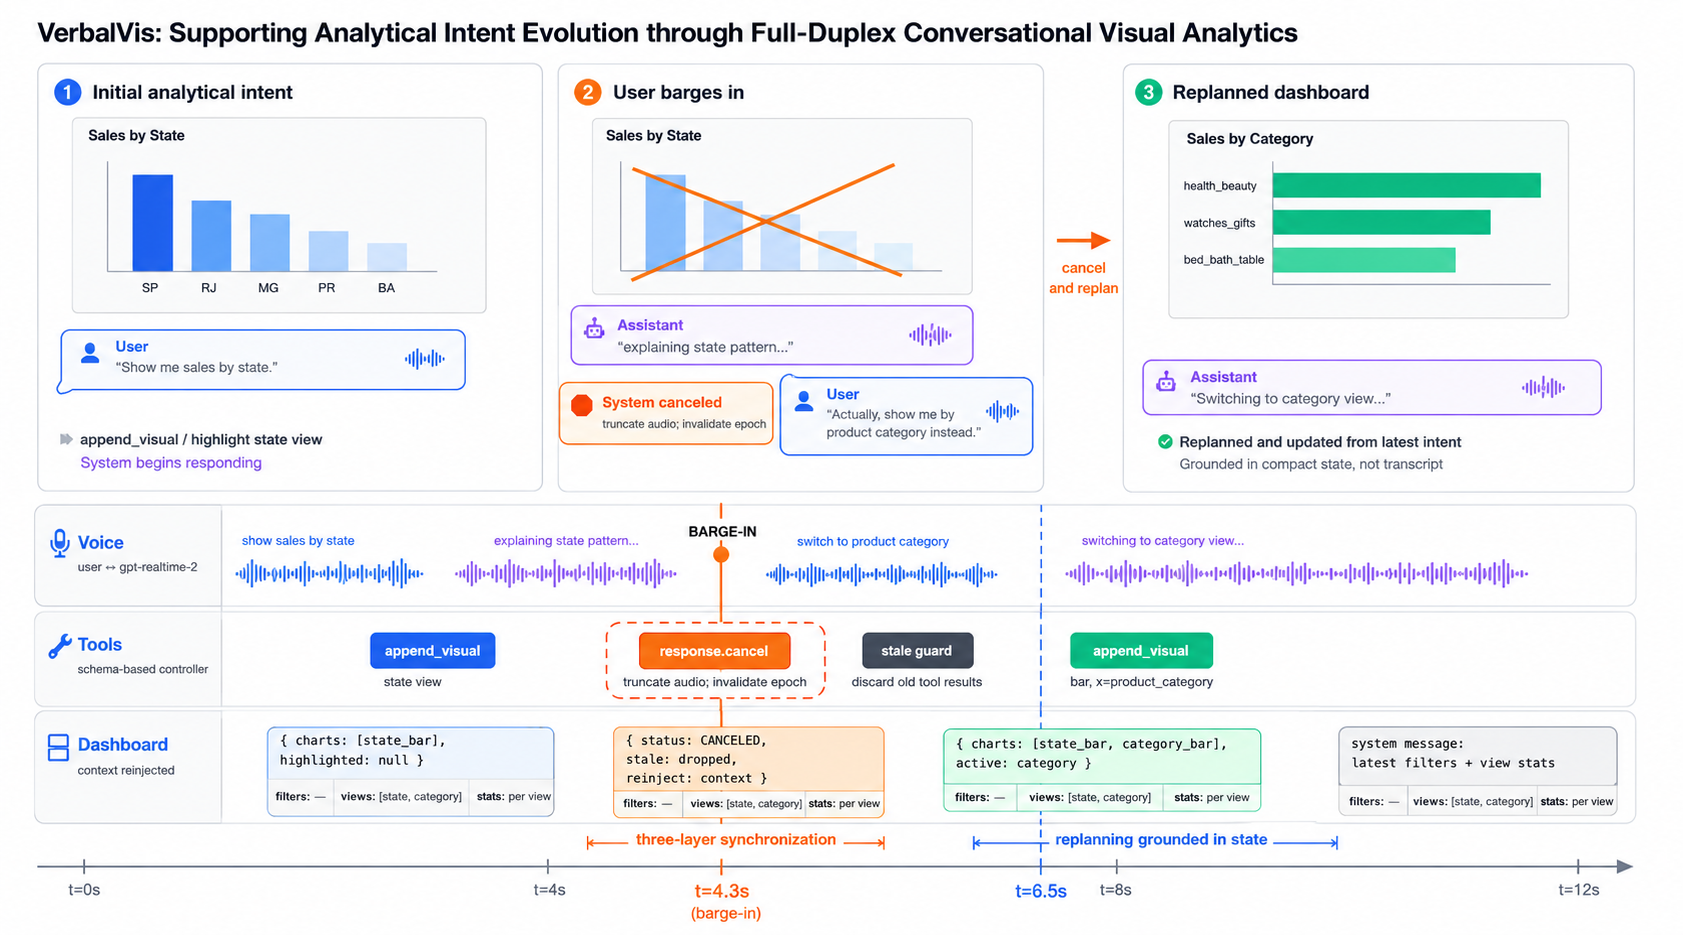
\includegraphics[width=\textwidth]{teaser-main.png}
\captionof{figure}{Overview of a barge-in episode in VerbalVis. While the assistant is explaining a visualization, the user interrupts to redirect the exploratory analysis from sales by state to sales by product category. VerbalVis immediately cancels obsolete speech, replans visualization actions through tool execution, reinjects the updated dashboard state as contextual grounding for the language model, and synchronously updates both the dashboard and spoken response. The aligned voice, tool, and dashboard timelines illustrate the coordinated full-duplex interaction that enables continuous analytical intent evolution without explicit turn switching.}
\label{fig:teaser}
\end{center}
}


\maketitle

% =====================================================================
% Abstract
% =====================================================================


\begin{abstract}
Exploratory data analysis is iterative: observations may cause analysts to
redirect their questions, revise provisional explanations, or change the data
scope under investigation. Existing speech- and language-driven visual
analytics systems generally support such revisions only after the current
response has completed. Full-duplex speech interaction allows users to redirect
an analysis while the assistant is still speaking, but stopping speech alone is
insufficient when the superseded response may also have initiated analytical
actions that modify a persistent dashboard. We present \textbf{VerbalVis}, a
full-duplex conversational visual analytics system that coordinates spoken
output, schema-grounded tool execution, and dashboard state during
mid-response redirection. VerbalVis truncates obsolete speech, supersedes the
active response, invalidates response-bound analytical actions, rejects stale
results, and replans from the latest committed dashboard state. To describe
analytical redirection, we distinguish three theory-informed, non-exhaustive,
and potentially overlapping objects of revision: the analytical goal, a
working hypothesis, and the analytical scope. These constructs guide design
inquiry and behavioral coding rather than runtime classification. A lightweight
formative inquiry informed requirements for cross-layer cancellation,
state-grounded replanning, and visible execution feedback. We evaluate
VerbalVis through an illustrative scenario and an exploratory within-subjects
study comparing full-duplex and turn-based conversational visual analysis.
\end{abstract}

\begin{IEEEkeywords}
Visual analytics, conversational interfaces, speech interaction, full-duplex
dialogue, analytical intent revision, exploratory data analysis.
\end{IEEEkeywords}
\section{Introduction}
\label{sec:intro}

\IEEEPARstart{E}{xploratory} data analysis (EDA) is inherently iterative.
Analysts rarely follow a fully specified plan; instead, they move among
observations, questions, tentative explanations, and new analytical actions as
evidence emerges. Patterns and anomalies can expose limitations in the current
direction and prompt analysts to reconsider what they are asking, what they
believe, or which data are relevant
\cite{russell1993cost,pirolli2005sensemaking,
sacha2014knowledge,battle2019characterizing}. We use
\emph{analytical intent revision} to denote an episode in which an analyst
supersedes, qualifies, or materially changes an active analytical commitment.

Natural-language interfaces and LLM-powered visual analytics systems
increasingly support contextual queries, visualization generation,
conversational refinement, and multistep analytical tool use
\cite{gao2015datatone,setlur2016eviza,narechania2021nl4dv,
dibia2023lida,wang2024dataformulator2,zhao2024lightva}. These capabilities make
it easier to express complex analytical requests and iteratively refine visual
results. However, refinement is generally organized around completed turns: a
user submits a request, the system produces an explanation or executes a
sequence of analytical actions, and the user changes direction only after that
response has finished. This organization is particularly restrictive for
speech, where system output unfolds over time and an analyst may recognize a
misdirected analysis well before the assistant has finished speaking. The
interaction therefore delays the system's response to a change that has already
occurred in the analyst's reasoning.

Full-duplex interaction provides a different regime by allowing the system to
continue listening while speaking. An analyst can redirect an ongoing analysis
through barge-in rather than waiting for a turn boundary. Yet barge-in alone
does not solve the visual analytics problem. Barge-in is a temporal event, not
necessarily evidence of analytical revision: a user may interrupt to correct
recognition, request clarification, acknowledge the assistant, or stop an
overly long response. More importantly, stopping speech does not necessarily
stop the analytical consequences of the superseded response. Analytical tool
actions and pending dashboard updates may continue after the user has changed
direction, and late results may still modify the visible state. The assistant
could therefore acknowledge the revised request while the dashboard continues
evolving according to the obsolete one. Full-duplex conversational visual
analytics consequently introduces a cross-layer consistency problem spanning
spoken output, analytical execution, and persistent dashboard state.

We present \textbf{VerbalVis}, a full-duplex conversational visual analytics
system designed to keep these layers aligned during mid-response redirection.
VerbalVis combines real-time speech interaction, schema-grounded analytical
tools, and a persistent dashboard through a visual-analytics-specific
orchestration layer. When a new request supersedes an active response, the
system truncates obsolete speech and advances a response-bound execution epoch.
Tool actions remain associated with the response that produced them; actions
and results from earlier epochs are treated as stale and cannot commit changes
to the dashboard. The revised request is then interpreted against the latest
committed dashboard state, including active filters, highlights, and
visualizations, so that replanning begins from what the analyst currently sees
rather than from speculative work associated with the cancelled response.
VerbalVis does not introduce a new speech model or interruption detector. Its
contribution is the response-supersession mechanism that coordinates speech
cancellation, analytical validity, and dashboard-grounded replanning.

Drawing on research in sensemaking and exploratory analysis, we characterize
analytical revisions through three potentially overlapping objects of change:
the analytical goal, a working hypothesis, and the analytical scope
\cite{pirolli2005sensemaking,klein2007dataframe,
bates1989berrypicking,battle2019characterizing}. These constructs provide a
vocabulary for describing how an active investigation is redirected, but they
do not imply that every interruption constitutes a revision or that every
revision belongs to only one category. They serve as theory-informed
sensitizing concepts and post-hoc coding dimensions rather than an exhaustive
taxonomy or runtime intent classes. A lightweight formative inquiry refined
their operational boundaries and informed requirements for cancellation, state
preservation, visible feedback, and recoverable dashboard interaction.

We evaluate VerbalVis through an illustrative usage scenario and an exploratory
within-subjects mixed-methods study with eight participants. The study compares
a \emph{Full-Duplex} condition, in which participants may redirect the assistant
while it is speaking, with a matched \emph{Turn-Based} condition, in which they
must wait for the current response to finish. We examine interaction
responsiveness, perceived control, state consistency, workload, exploratory
behavior, and analytical outcomes, with particular attention to when
participants revise an ongoing analysis and what they expect the system to
cancel, preserve, and update.

\textbf{Contributions.}
\begin{enumerate}
\setlength{\itemsep}{1pt}
\setlength{\parskip}{0pt}

\item A design framing for overlapping user speech in full-duplex
conversational visual analytics. We distinguish non-interruptive backchannels
from floor-taking barge-ins and characterize analytical revisions through
changes to analytical goals, working hypotheses, and analytical scope.

\item \textbf{VerbalVis}, a full-duplex conversational visual analytics system
that coordinates assistant speech, analytical tool execution, and persistent
dashboard state when an active analytical response is superseded. It supports
speech truncation, response-bound tool execution, stale-result rejection, and
replanning from the latest committed dashboard state.

\item An exploratory mixed-methods comparison of full-duplex and turn-based
speech interaction during open-ended visual analysis, examining
responsiveness, perceived control, interaction flow, state understanding,
workload, exploratory behavior, and analytical outcomes.

\end{enumerate}



\section{Related Work}
\label{sec:related}

VerbalVis connects research on natural-language interaction for visualization,
LLM-powered visual analytics, full-duplex spoken dialogue, and analytical
sensemaking. We review how these areas support conversational refinement,
analytical steering, interruption, and changes to an ongoing investigation.

\subsection{Natural-Language Interaction for Visualization}
\label{sec:rw-nli}

Natural-language interfaces for visualization translate utterances into data
attributes, analytical tasks, and visual specifications. DataTone exposes
alternative interpretations through interactive ambiguity widgets
\cite{gao2015datatone}, while Eviza grounds language in both the dataset and
the active visualization to support contextual references and follow-up
questions~\cite{setlur2016eviza}. NL4DV provides a reusable pipeline for
extracting attributes and analytical tasks and generating candidate
visualizations~\cite{narechania2021nl4dv}. These systems establish language
grounding, ambiguity management, and contextual interpretation as central
requirements for conversational visual analysis.

Multimodal systems extend this interaction by combining language with visible
references and direct manipulation. Orko integrates speech and touch for
network exploration~\cite{srinivasan2018orko}; InChorus characterizes
operations expressed through speech, pen, and touch
\cite{srinivasan2020inchorus}; and DataBreeze interweaves speech with direct
manipulation over flexible unit visualizations
\cite{srinivasan2021databreeze}. Snowy and conversational extensions of
NL4DV further support follow-up utterances and modification of existing views
\cite{srinivasan2021snowy,mitra2022conversational}. However, these systems
generally organize refinement around completed user and system turns.
VerbalVis instead considers redirection while speech and associated analytical
actions are still unfolding.

\subsection{LLM-Powered and Agentic Visual Analytics}
\label{sec:rw-agentic}

Large language models extend conversational visualization beyond mapping one
utterance to one chart. LIDA decomposes visualization generation into data
summarization, goal generation, chart creation, and evaluation
\cite{dibia2023lida}. Data Formulator combines natural-language concepts with
directly specified visual encodings, while Data Formulator~2 supports iterative
authoring and navigation through alternative data and visualization histories
\cite{wang2024dataformulator,wang2024dataformulator2}. These systems broaden
the role of language from chart specification to data transformation and
iterative visual design.

Agentic systems further delegate analytical planning and execution to
LLM-based components. InsightPilot and LightVA translate higher-level
analytical goals into sequences of tasks, visualizations, and findings
\cite{ma2023insightpilot,zhao2024lightva}. WaitGPT externalizes intermediate
analysis operations for inspection and modification
\cite{xie2024waitgpt}, while InsightLens links conversation, code,
visualizations, and findings across an extended analysis
\cite{weng2025insightlens}. Such systems make analytical processes more
steerable and inspectable. Nevertheless, steering is usually performed through
subsequent prompts, graphical controls, or explicit checkpoints. Existing work
rarely specifies whether an unfinished action generated by an earlier response
remains valid after the user has redirected the analysis.

\subsection{Full-Duplex Dialogue and Interruption}
\label{sec:rw-duplex}

Streaming speech systems incrementally process or generate audio, whereas
full-duplex systems continue listening while speaking. They must distinguish
background speech, backchannels, cooperative overlap, and attempts to take the
conversational floor~\cite{skantze2021turntaking}. Barge-in has traditionally
referred to detecting user speech during system output and stopping or
modifying the active response~\cite{heins1997bargein}. Recent systems including
Duplex Conversation, SyncLLM, Moshi, and SALMONN-omni investigate concurrent
speech streams, low-latency turn-taking, and context-sensitive interruption
\cite{lin2022duplex,veluri2024syncllm,
defossez2024moshi,yu2025salmonnomni}.

Interruption timing, however, does not determine analytical meaning. A user may
interrupt to acknowledge the assistant, repair recognition, request
clarification, or revise the investigation. Conversely, an analyst may revise
the analysis after the assistant has finished speaking. Moreover, stopping
audio does not automatically cancel a database query, visualization tool call,
or pending dashboard update. VerbalVis therefore treats barge-in as a temporal
signal while separately managing the validity of response-dependent analytical
work and persistent visual state.


\subsection{Sensemaking and Analytical Revision}
\label{sec:rw-sensemaking}

Sensemaking research characterizes analysis as an iterative process in which
questions, explanations, and data focus evolve as evidence is encountered
\cite{russell1993cost,pirolli2005sensemaking,sacha2014knowledge}.
For \emph{Analytical Goal Shift}, information-seeking studies describe evolving
queries and the refinement of broad goals into focused analytical subtasks
\cite{bates1989berrypicking,vakkari2001changes,battle2019characterizing}.
For \emph{Working-Hypothesis Revision}, Data--Frame Theory and scientific
reasoning show that provisional explanations may be questioned or replaced
when observations conflict with prior expectations
\cite{klein2007dataframe,klahr1988dual,chinn1993anomalous}.
For \emph{Analytical Scope Refinement}, information-foraging and visualization
task frameworks distinguish analytical purpose from the data target and its
progressive restriction by population, variable, time, geography, category, or
granularity
\cite{pirolli1999information,brehmer2013multilevel,
wongsuphasawat2016voyager}.

These traditions provide theoretical support for the three forms, but do not
establish a universal, exhaustive, or mutually exclusive taxonomy. We therefore
treat them as theory-informed sensitizing concepts.
Section~\ref{sec:formative} presents participants' utterances as empirical
instances and specifies the coding boundaries adopted in this work; it does
not serve as the theoretical evidence that these forms of revision exist.




Across these areas, prior work supports contextual language interaction,
multistep analytical execution, spoken interruption, and evolving analytical
histories. VerbalVis connects these capabilities by coordinating the validity
of spoken output, analytical actions, and persistent dashboard state when an
unfolding response is superseded.






% =====================================================================
\section{System Design and Implementation}
\label{sec:system}

\subsection{Design Goals}
The framework yields three design goals:
\begin{itemize}
\item \textbf{DG1: Continuous intent revision.} Support revision at any moment, not only at turn boundaries.
\item \textbf{DG2: Rapid replanning after supersession.} Once an interruption is detected during assistant output, the system must prevent stale response work from committing, interpret the redirecting utterance, and re-plan against current dashboard state with minimal added latency.
\item \textbf{DG3: Dashboard--intent synchrony.} The shared dashboard must always reflect the latest applied operations and must serve as the canonical source of truth for the LLM, so that explanations are grounded in what the user sees rather than in the model's prior outputs.
\end{itemize}

\subsection{Architecture Overview}
VerbalVis comprises a Vue~3 + Vega-Lite frontend, a FastAPI backend with an in-memory DuckDB analytics layer, and a relay that bridges a browser WebSocket to the OpenAI Realtime WebSocket (Fig.~\ref{fig:arch}). The backend exposes a single \texttt{/ws} endpoint; on connection, it constructs a \texttt{RealtimeSession} that runs two concurrent async loops --- one forwarding client audio frames to OpenAI, one demultiplexing OpenAI events to the client and dispatching tool calls.

\begin{figure}[t]
\centering
\fbox{\parbox{0.92\linewidth}{\centering\small
\textbf{[Figure placeholder]} System architecture: Frontend (Vue/Vega-Lite) $\leftrightarrow$ Backend (FastAPI relay + DuckDB) $\leftrightarrow$ OpenAI Realtime (\texttt{gpt-realtime-2}). Realtime Layer (audio streaming, VAD, barge-in, response cancel) on the left; Analytics Layer (tool calls, DuckDB, dashboard update) on the right; shared dashboard state in the middle.}}
\caption{VerbalVis architecture. The Realtime Layer handles conversational coordination; the Analytics Layer executes tool calls asynchronously and updates the dashboard state, which is reinjected as system context after every tool call.}
\label{fig:arch}
\end{figure}

\noindent\emph{Realtime layer.} \texttt{gpt-realtime-2} streams 24\,kHz PCM audio in both directions. Depending on the experimental condition, the frontend uses local voice gating or push-to-talk, while the Realtime session may also expose server-side speech events such as \texttt{input\_audio\_buffer.speech\_started} and \texttt{\dots speech\_stopped}. On interruption-relevant events, the backend increments a \emph{turn epoch}, records the in-flight \texttt{response\_id} as invalidated, and marks tool tasks from the cancelled response as stale. In push-to-talk mode the backend additionally sends \texttt{response.cancel}; in server-interruption mode, it relies on the Realtime session's native interruption behavior and applies the same stale-result discipline locally.

\noindent\emph{Analytics layer.} Tool calls (\texttt{response.function\_call\_arguments.done}) are dispatched to handlers backed by DuckDB queries. DuckDB holds two derived fact tables built from seven Olist CSVs at startup: \texttt{fact\_order} (one row per delivered order, carrying order-grain attributes including \texttt{order\_month}, \texttt{review\_score}, \texttt{customer\_state}, \texttt{delivery\_days}, and per-order payment) and \texttt{fact\_item} (one row per order item, additionally carrying \texttt{product\_category} and per-item revenue $\textrm{price} + \textrm{freight}$). The two-table design lets revenue retain the correct semantics under both order-grain and item-grain aggregations; cross-grain filters on \texttt{product\_category} from the order table are rewritten as \texttt{order\_id IN (SELECT \dots FROM fact\_item WHERE \dots)} subqueries by a shared \texttt{build\_where} helper.

VerbalVis employs real-time full-duplex audio interaction for conversational coordination, while analytical operations are executed asynchronously through tool calls that update the dashboard state.

\subsection{Tool Taxonomy}
Following the Brehmer--Munzner multi-level typology~\cite{brehmer2013multi} and Yi et al.'s how-axis~\cite{yi2007toward}, we organize VerbalVis operations along three dimensions: \emph{why} (analytical goal), \emph{how} (interaction primitive), and \emph{what} (target of the operation: data, view, layout, insight). Table~\ref{tab:tools} lists a 15-operation taxonomy for the design space. The current prototype realizes five dashboard operations end-to-end as schema-based tools: \texttt{filter\_data}, \texttt{remove\_filter}, \texttt{highlight\_visual}, \texttt{append\_visual}, and \texttt{delete\_visual}. This subset is deliberately narrow: it covers the operations needed for the running example and user-study tasks while keeping tool selection predictable under realtime interruption.

\begin{table*}[t]
\centering
\caption{VerbalVis Tool Taxonomy. Five operations are implemented end-to-end as schema-based tools (marked $\checkmark$); the remainder define the broader design space. \emph{Why} follows Brehmer--Munzner; \emph{How} follows Yi et al.; \emph{What} identifies the operation target.}
\label{tab:tools}
\small
\begin{tabular}{lllllc}
\toprule
\textbf{Tool} & \textbf{Why} & \textbf{Why-Detail} & \textbf{How} & \textbf{What} & \textbf{Impl.} \\
\midrule
\texttt{filter\_data}          & Discover & Locate     & Filter                 & Data    & $\checkmark$ \\
\texttt{remove\_filter}        & Discover & Locate     & Filter                 & Data    & $\checkmark$ \\
\texttt{aggregate\_data}       & Discover & Summarize  & Abstract/Elaborate     & Data    &              \\
\texttt{compare\_data}         & Discover & Compare    & Connect                & Data    &              \\
\texttt{change\_chart\_type}   & Discover & Explore    & Encode                 & View    &              \\
\texttt{change\_encoding}      & Present  & ---        & Encode                 & View    &              \\
\texttt{change\_sort}          & Discover & Compare    & Reconfigure            & View    &              \\
\texttt{highlight\_visual}     & Discover & Locate     & Select                 & View    & $\checkmark$ \\
\texttt{focus\_visual}         & Discover & Explore    & Select+Reconfigure     & View    &              \\
\texttt{append\_visual}        & Discover & Explore    & Encode                 & View    & $\checkmark$ \\
\texttt{move\_visual}          & Present  & ---        & Reconfigure            & Layout  &              \\
\texttt{delete\_visual}        & Discover & Identify   & Reconfigure            & Layout  & $\checkmark$ \\
\texttt{replace\_visual}       & Discover & Explore    & Reconfigure            & Layout  &              \\
\texttt{explain\_visual}       & Discover & Identify   & Connect                & Insight &              \\
\texttt{summarize\_dashboard}  & Discover & Summarize  & Abstract/Elaborate     & Insight &              \\
\bottomrule
\end{tabular}
\end{table*}

\noindent The implemented tools are deliberately minimal. \texttt{filter\_data} centralizes global dataset narrowing (with a \texttt{field=null} convention for clearing, an \texttt{append} flag for AND-accumulation, and operator support for \texttt{eq, neq, in, gte, lte, between}); \texttt{remove\_filter} removes one field constraint without disturbing the rest; \texttt{highlight\_visual} redirects attention without changing data; \texttt{append\_visual} creates a new chart at item or order grain based on whether \texttt{product\_category} appears in the encoding; and \texttt{delete\_visual} removes views from the shared workspace. This minimality is intentional: most analytical state changes in our scenarios can be expressed by composing these operations, which keeps the model's tool-selection decision tree shallow and reduces the surface area on which the LLM can hallucinate.

\subsection{Layered Prompt Design}
The system prompt is constructed in four labeled sections, in line with the prompt-structure recommendations of the GPT-realtime-2 prompting guide~\cite{openai_realtime_prompt}. \emph{Identity} fixes the assistant as a collaborative data analyst, instructs language mirroring, and prescribes the opening behavior (greet, introduce the Olist dataset, walk through the four base views, then invite the user to choose a direction --- explicitly without preemptively highlighting any view). \emph{Dashboard Knowledge} provides a bidirectional view-id $\leftrightarrow$ Chinese-and-English-label dictionary, the exhaustive field list (forbidding fabricated fields such as ``return\_rate'' or ``profit''), and value semantics (e.g., \texttt{review\_score} 1--2 negative; \texttt{customer\_state} two-letter codes; revenue in BRL pronounced ``reais''). \emph{Tool Usage Rules} specify operator semantics, the cross-grain filter convention, and tool-selection guidelines that explicitly forbid defaulting to the review view for generic prompts such as ``what is interesting in the data.'' \emph{Realtime Rules} legitimize interruption as a high-priority signal and instruct the model to abandon prior explanations and re-evaluate against the latest user utterance.

\subsection{Dashboard State and Context Reinjection}
The four base views (\texttt{view-trend}, \texttt{view-review}, \texttt{view-map}, \texttt{view-category}) and any user-added \texttt{workspace-N} charts are maintained as a single backend list. After every tool call, the backend (i) re-queries all views against the current filter set, (ii) recomputes per-view summary statistics (e.g., peak month, low-score ratio, top state, top category), (iii) pushes a \texttt{views\_update} event to the frontend for re-render, and (iv) injects a compact textual snapshot of the dashboard --- highlighted view, active filters, total filtered row count, and per-view summary --- back into the LLM as a \texttt{system} message. This \emph{context reinjection} pattern follows the guidance in the GPT-realtime-2 long-context section~\cite{openai_realtime_prompt}: the model is never asked to reconstruct dashboard state from prior turns, only to act on what it is given.

\subsection{Supersession Control Protocol}
VerbalVis treats barge-in as a control event, not as a semantic classifier. The reusable protocol has five stages. First, the runtime detects possible supersession through either a server speech-start event or a client push-to-talk start during assistant output. Second, the backend increments \texttt{turn\_epoch}, so newly arriving user input and later tool calls belong to a new response epoch. Third, the system attempts to stop obsolete output through \texttt{response.cancel} or \texttt{conversation.item.truncate}, depending on the input mode and Realtime event sequence. Fourth, tool calls associated with the superseded response are cancelled when possible and otherwise checked with \texttt{is\_stale\_tool\_call} before any result is returned to the model or applied to the dashboard. Fifth, VerbalVis reinjects a compact dashboard snapshot before the next \texttt{response.create}, so the revised plan is grounded in the latest valid visual state.

When barge-in is enabled, an interruption is represented by either a server speech-start event or a client push-to-talk start during assistant output. The backend then:
\begin{enumerate}
\item Increment the per-session \texttt{turn\_epoch}; record the in-flight \texttt{response\_id} as invalidated.
\item Cancel all in-flight tool tasks bound to the cancelled response.
\item Send \texttt{response.cancel} or \texttt{conversation.item.truncate} when the local input mode requires explicit cancellation or audio truncation.
\item Forward \texttt{speech\_started} to the frontend so the UI can stop playback immediately.
\end{enumerate}
A double-lock discipline (\texttt{openai\_send\_lock} for outbound messages, \texttt{tool\_state\_lock} for state mutation) and a per-response pending-tool counter ensure that (i) tool results from cancelled responses are discarded by an \texttt{is\_stale\_tool\_call} check before being forwarded to the model, and (ii) when a single model turn issues multiple tool calls, only the final completing call triggers a fresh \texttt{response.create}, preventing duplicate or racing responses.

\noindent\textbf{No-barge ablation.}
We define \textbf{VerbalVis-NoBarge} as the controlled ablation of the protocol. It uses the same \texttt{gpt-realtime-2} model, voice, prompt, tool schema, dashboard, backend, VAD settings, and context-reinjection logic as VerbalVis-FullDuplex. The only intended difference is policy: user speech during assistant output is recorded or queued, but it does not trigger \texttt{response.cancel}, \texttt{conversation.item.truncate}, epoch invalidation, or stale-tool discard until the current response completes. This condition separates the effect of the realtime model family from the specific effect of the supersession path.

% =====================================================================
\section{Case Study: Three Forms of Analytical Intent Revision}
\label{sec:case}

We illustrate the framework with a single session on the Olist Brazilian e-commerce dataset (96{,}478 delivered orders; 110{,}196 order items spanning 73 product categories and 27 states; September 2016 -- August 2018). The analyst, a domain non-expert, was asked to explore customer satisfaction with no predetermined goal.

\subsection{Initial State} The system greets the user, names the dataset, and walks through the four base views: monthly order trend, review-score distribution, orders by state, top-15 categories by revenue. The system then asks the analyst what they would like to explore. The analyst responds, ``Let's look at the trend.''

\subsection{Type 1 --- Goal Shift}
\emph{System (mid-utterance):} ``Order volume peaks in November 2017, roughly 4$\times$ the average month. Let me decompose that by product category to see whether it's a Black Friday effect across categories or concentrated in --- ''
\emph{Analyst (barge-in):} ``I care more about ratings, not sales.''

The barge-in fires \texttt{response.cancel}; the redirecting utterance is interpreted; the controller emits \texttt{highlight\_visual(view-review)} and the assistant continues: ``The review distribution is heavily concentrated at 5 stars but with a non-trivial 1- and 2-star tail. Want me to filter to low-rated orders and see what they share?'' The intent has shifted from a sales decomposition to a satisfaction investigation; the analyst was spared the remainder of the category breakdown.

\subsection{Type 2 --- Hypothesis Correction}
\emph{System (mid-utterance):} ``Electronics-adjacent categories such as \texttt{computers\_accessories} and \texttt{electronics} show below-average ratings. This is often attributable to product quality issues with --- ''
\emph{Analyst (barge-in):} ``It's logistics, not the products.''

The system invokes \texttt{append\_visual(scatter, delivery\_days, review\_score)} followed by \texttt{filter\_data(review\_score, lte, 2)}; the resulting scatter shows the low-rated tail clustering at high delivery days. The assistant continues: ``You're right --- low-rated orders disproportionately have delivery times above 20 days; the product-quality story doesn't hold up.'' The intent revision substituted a delivery hypothesis for a product-quality hypothesis, and the assistant aborted its prior explanation rather than completing it.

\subsection{Type 3 --- Scope Narrowing}
\emph{System (mid-utterance):} ``Among states with the worst delivery times, the northeast --- Bahia and Cear\'a --- have averages above 25 days, while --- ''
\emph{Analyst (barge-in):} ``Just S\~ao Paulo.''

\texttt{filter\_data(customer\_state, eq, "SP")} is issued; all four base views recompute against the SP-only subset; the assistant pivots to ``Within SP, average delivery is 8.4 days; the low-rated tail is much smaller than the national figure.'' Scope contracted from a national survey to a state-level focus, exploiting the analyst's prior interest in SP without the analyst having had to articulate that interest at the start of the session.

\subsection{Summary}
Each revision corresponds to one of the three framework types; the dashboard, the system narration, and the model's working hypothesis remained synchronized throughout because every superseded response was followed by a fresh \texttt{conversation.item.create} of dashboard context before the next \texttt{response.create}. We argue this synchrony is the practical value of treating barge-in as a structural supersession signal rather than merely as audio cancellation.

% =====================================================================
\section{User Study and Technical Benchmark}
\label{sec:study}

\subsection{Design}
The study is designed to test the paper's central claim rather than general usability: whether a full-duplex supersession pathway makes analytical intent revision in EDA faster, more natural, and more controllable. The primary causal comparison is \textbf{not} between a realtime speech model and a cascaded speech pipeline. Instead, we compare two conditions that share the same model, voice, prompt, tool schema, dashboard, backend, VAD configuration, and context-reinjection logic. The only intended difference is whether user speech during assistant output triggers immediate response cancellation, epoch invalidation, and stale-action discard.

We plan a within-subjects, counterbalanced study with $N{=}12$--$16$ participants. Participants must have basic data-analysis experience, but need not know the Olist domain in advance. Each participant completes two open-ended exploration tasks on the Olist dataset, one per primary condition; task--condition assignment and condition order are counterbalanced. Each task lasts 12--15 minutes after a short tutorial.

\begin{itemize}
\item \textbf{Condition A (VerbalVis-FullDuplex):} audio is handled by the \texttt{gpt-realtime-2} session; the user can speak during assistant output; barge-in cancels or truncates the current response, increments \texttt{turn\_epoch}, invalidates stale tool work, and triggers replanning against reinjected dashboard context.
\item \textbf{Condition B (VerbalVis-NoBarge):} the system uses the same \texttt{gpt-realtime-2} session, voice, prompt, VAD settings, dashboard, backend, tool schema, and context-injection logic. However, user speech during assistant output is queued until the current response completes; it does not trigger \texttt{response.cancel}, \texttt{conversation.item.truncate}, immediate epoch invalidation, or stale-tool discard. This preserves the realtime model family while removing the supersession policy.
\end{itemize}

\noindent\textbf{Supplementary ecological baseline.}
We additionally define \textbf{VerbalVis-Cascade} as an ecological baseline rather than the main causal comparison. In this condition, user speech is transcribed by ASR, passed to a text LLM using the same dashboard tool schema and Olist backend, and synthesized back to speech with TTS. The user must wait for the system to finish before the next request is processed. This baseline represents the speech-wrapped, turn-based text-LLM VA regime implicit in systems such as LightVA and DashChat, but it necessarily changes model type, speech pipeline, ASR/TTS latency, audio quality, turn-taking policy, and response timing. We therefore report Cascade results as supplementary context, not as evidence that the barge-in mechanism alone caused any observed advantage.

\subsection{Tasks}
Tasks are written to invite open-ended EDA while naturally eliciting the three revision types in our framework. Participants are not instructed to interrupt. The tutorial only explains the interaction regime of each condition: in FullDuplex they may speak whenever they want to redirect the analysis; in NoBarge their speech during assistant output is accepted but processed after the current response finishes. If Cascade is run, participants are told that it is a turn-based speech interface whose next request is processed only after the current response completes.

\begin{itemize}
\item \textbf{Customer satisfaction task.} ``Explore what factors may be associated with low customer review scores. Produce three findings and one follow-up recommendation.''
\item \textbf{Sales, logistics, and region task.} ``Investigate unusual order or revenue patterns and whether they relate to delivery or regional differences. Produce three findings and one follow-up recommendation.''
\end{itemize}

\subsection{Measurements}
\textbf{Quantitative.}
\begin{itemize}
\item \emph{Intent revision count} --- number of user-initiated direction changes per session, coded from session video, transcript, dashboard events, and the \texttt{barge\_in.log} timeline.
\item \emph{Revision type distribution} --- proportion of revisions coded as Goal Shift, Hypothesis Correction, or Scope Narrowing.
\item \emph{Exploration breadth} --- number of distinct analytical dimensions touched (fields, views, filter expressions) during the session.
\item \emph{Insight count} --- number of substantive findings reported in the post-task summary, coded by two raters with Cohen's $\kappa$ reported.
\item \emph{Time-to-revision} --- elapsed time between the start of the redirecting utterance and the first system action aligned with the new intent, measured from video and event logs.
\item \emph{Wasted output time} --- time during which the system continues producing the old analytical direction after the participant has begun redirecting.
\item \emph{Queue delay} --- in NoBarge, the interval between redirecting speech onset and the moment the queued request begins processing.
\item \emph{Time-to-first-audio (TTFA)} and \emph{tool-call duration}, recorded automatically by the existing \texttt{\_response\_metrics} instrumentation in \texttt{realtime.py}; if Cascade is run, ASR, text-LLM, and TTS latencies are logged separately and reported as component-level ecological costs.
\end{itemize}

\textbf{Qualitative.}
\begin{itemize}
\item Think-aloud transcripts, coded thematically.
\item Semi-structured post-task interviews (10--15 min).
\item NASA-TLX (six standard sub-scales).
\item Perceived Control scale (3 Likert-7 items, e.g., ``I felt able to redirect the analysis whenever I wanted.'').
\end{itemize}

\subsection{Episode Coding}
The unit of analysis is a \emph{revision episode}. Two coders inspect synchronized transcripts, screen recordings, dashboard event logs, and audio timelines. For each candidate episode, coders determine (i) whether it is a valid analytical intent revision rather than a clarification, backchannel, or unrelated speech fragment; (ii) whether it is Goal Shift, Hypothesis Correction, or Scope Narrowing; (iii) whether the system successfully responded to the revised intent; and (iv) the time from the start of the redirecting utterance to the first aligned system action, such as a tool call, dashboard update, or explicit spoken acknowledgment. Disagreements are resolved through discussion after reporting inter-rater agreement.

\subsection{Hypotheses}
\begin{itemize}
\item \textbf{H1:} Intent revision count is higher under VerbalVis-FullDuplex than under VerbalVis-NoBarge.
\item \textbf{H2:} VerbalVis-FullDuplex reduces time-to-revision, queue delay, and wasted output time relative to VerbalVis-NoBarge.
\item \textbf{H3:} VerbalVis-FullDuplex increases exploration breadth and insight count relative to VerbalVis-NoBarge.
\item \textbf{H4:} Perceived control is higher under VerbalVis-FullDuplex, while NASA-TLX is not significantly higher.
\item \textbf{H5:} The advantage of VerbalVis-FullDuplex is largest for \emph{Hypothesis Correction} and \emph{Scope Narrowing}, because these revisions are most costly when users must wait through an explanation they already intend to reject or constrain.
\end{itemize}

\subsection{Technical Benchmark}
To separate mechanism-level behavior from participant variability, we additionally plan a 250-trial automated benchmark comparing VerbalVis-FullDuplex and VerbalVis-NoBarge. Scripted audio scenarios cover five interruption families: no interruption, early goal shift, late goal shift, hypothesis correction, and scope narrowing. Each scenario is repeated across multiple seeds and dashboard states. The benchmark reports speech-onset detection latency, cancel/truncation latency, stale-tool discard rate, queued-request delay, post-supersession tool correctness, dashboard-context consistency, and component-level latency. The user study tests whether supersession-enabled full-duplex interaction changes analytical behavior and perceived control; the technical benchmark tests whether the mechanism itself reliably cancels stale work, discards stale calls, and preserves dashboard-context consistency.

\subsection{Results (to be reported)}
\emph{Placeholder.} Tables and figures will report per-condition means and within-subject differences for the primary FullDuplex--NoBarge comparison with Wilcoxon signed-rank tests and effect sizes. Cascade, if collected, will be reported in a separate supplementary table to contextualize ecological latency and user experience, not to support the causal barge-in claim. Qualitative themes will be illustrated with representative quotations. The instrumentation already in place yields TTFA, per-turn latency, tool-call duration, stale-call status, and a per-session dashboard context snapshot for every tool invocation, providing both quantitative and trace data.

\subsection{Anticipated Discussion}
We expect the analyses to show that (a) the three revision types in our framework appear in the data with distinguishable distributions across participants; (b) the FullDuplex advantage over NoBarge is largest on Hypothesis Correction and Scope Narrowing episodes, where delayed processing forces users to passively witness explanations they already intend to reject or constrain; and (c) Perceived Control correlates positively with intent revision count and negatively with wasted output time. We further expect the automated benchmark to show that the gain is not merely due to the realtime model family, but to the supersession pathway that cancels stale output and preserves dashboard-context consistency.

% =====================================================================
\section{Discussion}
\label{sec:discussion}

\textbf{Limitations.} The current prototype implements five of the fifteen taxonomy operations as schema-based tools; while these operations cover the running example and planned study tasks, claims about the taxonomy's completeness require broader deployment. VerbalVis treats all barge-in events with the same downstream processing and does not classify revision type at runtime; the three types in Section~\ref{sec:framework} are analytical categories, not separate system policies. The planned study size ($N{=}12$--$16$) is appropriate for an exploratory within-subjects system study but still limits statistical power for subgroup analysis. VerbalVis-NoBarge is a controlled ablation rather than a naturally deployed product: it preserves the realtime model family while disabling immediate supersession, which is useful for causal attribution but less ecologically familiar. Conversely, VerbalVis-Cascade is ecologically meaningful because it represents a speech-wrapped text-LLM VA regime, but it changes model type, speech pipeline, latency decomposition, audio quality, and turn-taking policy; we therefore treat it only as supplementary context. Finally, the Olist dataset, while rich, is domain-specific; generalization to clinical, financial, or scientific datasets remains future work.

\textbf{Implications.} Treating barge-in as a structural supersession signal expands the conversational VA design space without requiring the system to infer the user's meaning from timing alone. The interruption event gives the controller permission to protect the analytical state from stale work; the redirecting utterance provides the content of the revised intent. Future systems may also use the \emph{timing} of an interruption (early vs.\ late in a response) as a weak cue about whether the user rejects the direction, the evidence, or the conclusion, but such use should remain subordinate to the utterance content and dashboard context.

\textbf{Generalization beyond voice.} The framework is voice-motivated but not voice-bound. Any modality with a true interruption primitive --- including streaming-LLM text chat with mid-response edits, or gestural systems that can preempt animations --- can be analyzed through the same Intent Evolution lens. We see VerbalVis as a concrete instantiation of a broader design pattern.

\textbf{Future work.} Beyond completing the tool taxonomy and broadening data domains, we plan (i) type-aware interruption handling that differentiates Goal Shift, Hypothesis Correction, and Scope Narrowing at runtime, (ii) a longitudinal study examining whether users' intent-revision strategies stabilize over repeated sessions, and (iii) an extension to multi-analyst sessions where barge-ins from different participants might conflict or require negotiated replanning.

% =====================================================================
\section{Conclusion}
\label{sec:conclusion}
We have presented VerbalVis, a full-duplex conversational visual analytics system motivated by the observation that user barge-in can serve as a structural supersession signal during analytical work. The Intent Evolution framework identifies three recurring revision types --- Goal Shift, Hypothesis Correction, and Scope Narrowing --- and motivates a reusable supersession control protocol for conversational EDA. Built on \texttt{gpt-realtime-2}, response epochs, schema-based tool calling, and an in-memory DuckDB analytics layer with continuously reinjected dashboard context, VerbalVis demonstrates how full-duplex speech can move intent revision from a between-turn afterthought to a continuously available action. A case study on the Olist e-commerce dataset illustrates all three revision types in a single session; a planned within-subjects user study will make its primary comparison between VerbalVis-FullDuplex and VerbalVis-NoBarge, with VerbalVis-Cascade retained only as a supplementary ecological baseline; and a 250-trial technical benchmark will test the reliability of the supersession mechanism. Together, these evaluations separate the human effect of full-duplex redirection from the mechanism-level question of whether stale work can be canceled or discarded while dashboard context remains consistent.

% =====================================================================
\bibliographystyle{IEEEtran}
\bibliography{main}

\end{document}
 
